\chapter{\acl{fra}} \label{sec:haupt}
In diesem Kapitel soll auf die  Vorgehensweise und die Implementierung des in \ref{sec:thema} vorgestellte \ac{fra} eingegangen werden. schwerpunkte.... In dieser Arbeit wird nur die \acl{xbar} softwareseitig implementiert, da es sonst den Umfang der Arbeit übersteigt.

%Aktuelle Implementierung
%Theoretische Grundlagen o.ä.
%Umsetzung

\section{Generischer Plattformtreiber} \label{sec:plat}
Um eine einwandfreie Kommunikation zwischen den Firmware Modulen im \ac{fpga} und dem Kernel zu gewährleisten, muss ein generischer Treiber erstellt werden. 


Wie in dem Kapitel~\ref{sec:plat_t} bereits erläutert, werden für die grundlegende Funktionsweise eines Treiber verschiedene Funktionen benötigt. Zunächst soll auf die Registrierungs- bzw. Aufräumfunktion des Treibers eingegangen werden.\\


Beim Laden des Treibers werden verschiedene allgemeingültige Parameter gesetzt und zusätzlich Speicherplatz allokiert. 
\begin{lstlisting}
struct afm_driver
{
	unsigned int major_id;

	uint8_t minor_list[AFM_MAX];
	spinlock_t minor_spinlock;
	struct class * class;
};
\end{lstlisting}
\captionof{code}{\label{code:afm_data}Struktur des Treibers}

Im Treiber wird beim Laden als Erstes eine Klasse erstellt, der später die einzelnen Module zugeordnet werden. Diese Klasse wird in der dem Treiber zugehörigen Struktur \textit{afm\_driver} in der Variablen \textit{class} abgespeichert. 


Da die Majornummer den Treiber kennzeichnet (siehe Kapitel~\ref{sec:mmnum_t}) wird diese in der globalen Treiberstruktur als \textit{major\_id} gespeichert. Für die Minornummer wird in der Datenstruktur eine Liste \textit{minor\_list[AFM\_MAX]} und ein zugehöriges Spinlock \textit{minor\_spinlock} initialisiert. Über die Liste wird später eine freie Nummer ausgewählt, die bei jedem Gerät individuell ist und gleichzeitig wird dadurch die Anzahl der möglichen Module auf \textit{AFM\_MAX} begrenzt. Das Spinlock sorgt bei der Auswahl der Minornummer für einen unterbrechungsfreien Vorgang, sodass keine Nummer doppelt vergeben werden kann. 


Am Ende der initialen Funktion wird der Plattformtreiber mit der \textit{platfrom\_driver} Struktur (siehe Codebeispiel~\ref{code:platform_driver}) registriert. Damit werden die initiale Funktion zum Anlegen, aber auch die Funktion zum Deinitialisieren der Geräte übergeben.


Analog wird beim Freigeben des Treibers der allokierte Speicherplatz freigegeben, der Plattformtreiber abgemeldet und die erstelle Klasse zerstört.\\


Beim Anlegen einer Instanz vom Treiber wird die \textit{.probe} Funktion aufgerufen und zusätzlich wird der Modultyp und Name in einer \textit{arri\_fra\_mod\_config} Struktur zur Verfügung gestellt.
%todo aussotieren
\begin{lstlisting}
struct afm_device 
{
	struct arri_fra_mod_config *mod_config;
	
	struct class *class;
	struct cdev cdev;
	unsigned int minor_id;
	struct platform_device *pdev;
	struct resource *res;
	u8 __iomem *base;
	
	struct afm_file fdev[AFM_FILE_MAX];
	spinlock_t open_spinlock;
	%atomic_t use_count;
	
	#define AFM_NOLOGGING   ((uint32_t)0U)
	#define AFM_LOGGING     ((uint32_t)1U)
	uint32_t has_logging;
};
\end{lstlisting}
\captionof{code}{\label{code:afm_device}Auszug aus der Struktur einer Instanz}

In der initialen Funktion der Instanz wird diese Struktur genutzt um spezifische Einstellungen für jede einzelne Instanz festgelegt und in einer entsprechenden Datenstruktur (siehe Codebeispiel~\ref{code:afm_device}) gespeichert. 


Der einzige Übergabeparameter der Probefunktion ist die Struktur des \textit{platform\_device}, diese wird in dem Zeiger \textit{*pdev} gespeichert. Auch die, beim Laden des Treibers, angelegte Klasse wird ohne weitere Änderungen unter \textit{*class} abgelegt. 

Aus der Liste der Minornummern (siehe Codebeispiel~\ref{code:afm_data}) wird nach dem Sperren des zugehörigen Spinlocks eine freie Nummer ausgewählt und als \textit{minor\_id}, sowie auf verwendet gesetzt. 

Anschließend wird mit Hilfe der Majornummer und der Minornummer ein Device erstellt und als \textit{cdev} gespeichert. 

%todo vorteile statischer speicher
Damit das Öffnen der Devices auf eine bestimmte Anzahl limitiert ist, wird beim Initialisieren der Instanz ein Array der \textit{afm\_file} Struktur angelegt. Gleichzeitig wird der Speicherplatz statisch zur Kompilierzeit reserviert. Durch den Spinlock \textit{open\_spinlock} wird später dafür gesorgt, dass die Auswahl nicht unterbrochen und somit verfälscht wird.

%todo base/res

\section{Konzeptionierung der \acl{ioctl}s}\label{sec:ioctl}
%todo zu oft ioctl
%über ioctl zugriff auf das geöffnete Device
%Auf die ioctl eingehen und die Überlegungen hinter diesen
%hello, logging/unlogging?, get id, get reg, get reg bitmask, get reg block, set reg, set reg bitmask, set reg block, 
In dem Abschnitt soll auf die Konzeptionierung der \ac{ioctl}s eingegangen werden. Wie in Kapitel~\ref{sec:ioctl_t} erläutert werden \ac{ioctl}s benötigt um zwischen Kernel und Userspace Daten auszutauschen. Da der Großteil der Software im Userspace läuft, aber der Treiber im Kernel, wird der hauptsächliche Zugriff auf die Geräte über \ac{ioctl}s geregelt.\\


Als Erstes ist eine Anmeldung der Anwendung bei dem Gerät notwendig. Um die Eindeutigkeit zu garantieren wird hier die \ac{pid} übergeben. Allerdings wird auch der Prozessname benötigt, damit eine schnelle Nachvollziehbarkeit vorhanden ist. Wie in Kapitel~\ref{sec:konzept} erläutert, soll die Unterscheidung zwischen Standardapplikation und Debugtool möglich sein. Aus diesem Grund wird bei der Anmeldung zusätzlich zur \ac{pid} und dem Prozessnamen auch der Typ der Applikation übergeben. 
%todo satz hier oder wo anders?
Ohne die Ausführung von dem \textit{ARRI\_FRA\_MOD\_HELLO} \ac{ioctl} bleibt der weitere Zugriff auf das Gerät über \ac{ioctl}s verwehrt.\\

Die Protokollierung der Zugriffe auf ein Gerät ist ein notwendiger Bestandteil. Dadurch soll vor allem im Fehlerfall, die Suche erleichtert werden. Aufgrund der Zugriffe durch verschiedene Prozesse besteht ohne Protokollierung kein einheitlicher Überblick über diese.
In dem Zusammenhang werden zwei \ac{ioctl}s angelegt. Dabei ist \textit{ARRI\_FRA\_MOD\_LOGGING} zum Aktivieren der Protokollierung zuständig und analog wird diese durch \textit{ARRI\_FRA\_MOD\_NOLOGGING} deaktiviert. \\

Beim Anlegen des Geräts werden der Gerätetyp und der Name abgelegt. Im Userspace soll nach dem Öffnen des Geräts auf diese Informationen zugegriffen werden. Dafür wird ein eigenes \ac{ioctl} benötigt, welches den Typ und Namen aus der Instanzstruktur (siehe Codebeispiel~\ref{code:afm_device}) zurück gibt.\\

Die essenziellen Funktionen des Treibers sind das Setzen bzw. Auslesen von Register. Basierend auf den in der aktuellen Implementierung genutzten Funktionen und den entsprechenden Registerzugriffen, gibt es bis zu drei verschiedene Arten. Jede soll durch ein eigenes \ac{ioctl} abgebildet werden, da so die spätere Verwendung vereinfacht wird.  


Die Größe eines Registers ist auf 4 Byte normiert. Damit werden zum einfachen Setzen eines Registers lediglich zwei Parameter benötigt. Zum Einen die Stelle des Registers im Gerät(auch Registernummer) und zum anderen der Inhalt. 
Allerdings besteht auch die Notwendigkeit einzelne Bits oder mehrere hintereinander liegende Register über einen Aufruf zu setzen. Für beide gibt es ein gesondertes \ac{ioctl}. Zum Setzen von einzelnen Bits wird zusätzlich zu den beiden oben genannten Parametern noch eine Bitmaske übergeben. Mithilfe der Bitmaske werden im Register erst die entsprechenden Bits gelöscht und danach gesetzt. Dadurch ist es nicht notwendig erst über ein \ac{ioctl} das entsprechende Register auszulesen, anschließend im Userspace zu verändern und dann, wieder über ein \ac{ioctl}, in das gleiche Register zu setzen.
Der zweite Sonderfall benötigt andere Übergabeparameter als das einfache Setzen. Zusätzlich zu der Registernummer wird hier eine Registeranzahl gebraucht. Des Weiteren muss der Inhalt der Register in einem Array mit der Größe der Anzahl übergeben werden. Damit kann dann der Reihe nach jedes Register einzeln mit dem entsprechenden Inhalt beschrieben werden.


Das Auslesen der Register erfolgt nahezu analog zu dem Setzen. Der Parameter für den Registerinhalt wird hier allerdings über das \ac{ioctl} gefüllt und dann zurück in den Userspace übergeben. 
Register über eine Bitmaske auszulesen würde keine weiteren Vorteile gegenüber den Auslesen des ganzen Registers bieten. Aus diesem Grund wird es nicht implementiert.  
Damit man einen ganzen Block an Registern zurück lesen kann, muss durch das übergeben eines leeren Arrays mit der richtigen Größe der Speicherbereich zu Verfügung gestellt werden.\\

Dadurch sind die wichtigsten \ac{ioctl}s erläutert, die notwendig sind um die Grundfunktionen des Geräte abzudecken und zusätzlich eine triviale Debug Möglichkeit bieten.

\section{Implementierung im Kernel}\label{sec:kernel}
% Anlegen der Devices (arrifpga), Über Ioctl im Arri fpga treiber, öffnen und schließen des device, im eigenen Verzeichnis
% ioctl implementierung im kernel, was steht dahinter, wie funktioniert es, auszüge
Im Kernel gibt es zwei verschiedene Stellen, an welchen der Code implementiert ist. Zum einen muss der \ac{fpga} Treiber entsprechend erweitert werden, damit die Geräte unter Linux angelegt werden und zum anderen der \ac{fra} Treiber, um die angelegten Geräte zu Öffnen bzw. zu Schließen. \\

Zur besseren Übersichtlichkeit wurde sich für zwei Nameskonventionen entschieden. Strukturen und Funktionen, die mit \textit{arri\_fra\_mod} beginnen, werden außerhalb des \ac{fra} Treibers benötigt bzw. angelegt. Mit diesem Prefix werden die Namen recht lang, aus diesem Grund wird treiberintern auf den nicht so aussagekräftigen Prefix \textit{afm} abgekürzt.



%todo _static_assert mit aufnehmen

\subsection{Anlegen der Geräte}
%im fpga treiber
Der Zugriff der Software auf die \ac{fpga}-Module soll über Geräte stattfinden. Durch die unterschiedlichen Funktionalitäten der Module, wie in Kapitel~\ref{sec:bildkette} erläutert, werden diese Geräte als Kindgeräte vom \ac{fpga} angelegt, d.h. kernelseitig wird dieser Bestandteil im vorhandenen \ac{fpga} Treiber implementiert. 

\begin{lstlisting}
struct arri_fra_mod_init 
{
	#define ARRIFPGA_FRA_MAX_NAME   ((uint32_t)50)
	char type[ARRIFPGA_FRA_MAX_NAME];
	char name[ARRIFPGA_FRA_MAX_NAME];
	uint32_t offset;
	/* register size in bytes */
	uint32_t size;
};
\end{lstlisting}
\captionof{code}{\label{code:arri_fra_mod_init} Struktur zum Initialisieren des Geräts}

Über ein \ac{ioctl}, mit der obigen Struktur als Übergabeparameter, wird das Gerät angelegt. 


Als Erstes wird hier Speicherplatz für die drei Strukturen \textit{resource}, \textit{mfd\_cell} und \textit{arri\_fra\_mod\_config} allokiert. Mithilfe dieser am Ende der Funktion, die durch das \ac{ioctl} aufgerufen wird, das \ac{mfd} angelegt.


In der \textit{resource} Struktur (siehe Codebeispiel~\ref{code:res}) wird der Speicherbereich des \ac{fpga}-Modules abgebildet. Für die Variable \textit{start} wird auf den bereits allokierten \ac{fpga} Bereich noch der im \textit{arri\_fra\_mod\_init} übergebene \textit{offset} aufaddiert. Entsprechend ist wird für den \textit{end} Wert noch die \textit{size} addiert und zusätzlich eins abgezogen, da alles null basiert ist. Durch den Parameter \textit{flags} wird die Ressource als Speicherbereich festgelegt und als \textit{parent} wird die Ressource des gesamten \ac{fpga}s angegeben.


Als Nächstes wird die \textit{mfd\_cell} Struktur (siehe Codebeispiel~\ref{code:mfd_cell}) gefüllt. Hier wird die Variable \textit{id} auf eine globale Variable gesetzt, die bei jedem Funktionsaufruf um eins erhöht wird. \textit{num\_resources} wird auf eins gesetzt, da es für jedes Gerät nur eine Ressource gibt. Entsprechend wird in  \textit{resources} der aktuelle Zeiger der Ressource übergeben. Analog wird in \textit{platform\_data} der Zeiger auf die \textit{arri\_fra\_mod\_config} Struktur und in \textit{pdata\_size} die Größe der Struktur abgelegt.
Durch die \textit{arri\_fra\_mod\_config} wird der Gerätename und -typ an den Treiber übergeben.


Über die im Codebeispiel~\ref{code:mfd} aufgezeigt Funktionsdeklaration wird das Gerät angelegt. Dadurch wird die \textit{.probe} Funktion des Plattformtreibers ausgeführt und das erfolgreich angelegte Gerät ist auf der Kamera unter \textit{/dev/fra} zu finden.


\subsection{Öffnen und Schließen der Geräte}
%kernelseitige  implementierung im Treiber
Um später im Userspace auf die Geräte zuzugreifen und um initiale Einstellungen vorzunehmen, muss eine \textit{open} Methode implementiert werden. Im Umkehrschluss werden die Einstellungen durch die \textit{release} Funktion rückgängig gemacht. \cite[Seite 58f.]{corbet2005linux} \\

Die Anzahl von offenen Geräten ist durch die Speicherallokierung in der Struktur \textit{afm\_device} (siehe Codebeispiel~\ref{code:afm_device}) auf \textit{AFM\_FILE\_MAX} (hier: 4) begrenzt. Die geöffnete Instanz eines Geräts wird in der Struktur \textit{afm\_file} abgelegt.

\begin{lstlisting}
struct afm_file {  
#define AFM_FREE    ((uint8_t)0U)
#define AFM_USED    ((uint8_t)1U)
	uint8_t in_use;
	struct afm_device *dev;
	int minor;
	char name[ARRI_FRA_MOD_MAX_NAME];
	uint32_t type;
	uint32_t pid;
#define AFM_UNLOCK  ((uint32_t)0U)
#define AFM_LOCK    ((uint32_t)1U)
	uint32_t has_lock;
	struct file *file;
};
\end{lstlisting}
\captionof{code}{\label{code:afm_file} Struktur zum Ablegen des Geräts}
%todo caption umbenennen

Beim Öffnen eines Geräts wird, nachdem das entsprechende Spinlock (\textit{open\_spinlock}) gesperrt wurde, nach einem freien Gerät zum Öffnen gesucht. Hierzu wird über eine for-Schleife iteriert, bis die maximale Anzahl erreicht ist. In jedem Durchgang wird die Variable \textit{in\_use} überprüft, entsprechend dem Define kann dann festgestellt werden, ob es noch möglich ist ein Gerät zu öffnen. Wurde eine freie Stelle gefunden, wird der Parameter auf \textit{AFM\_USED} gesetzt und das Spinlock wieder freigegeben.
Wenn die maximale Anzahl erreicht ist, wird eine Fehlermeldung ausgegeben und ein Fehlercode zurückgehen.
Die Variable \textit{dev} wird auf das geöffnete Gerät gesetzt, analog wird \textit{minor} auf die verwendete Minornummer und \textit{file} auf die, in der \textit{open} Methode, übergebene Datei gesetzt. 
\textit{has\_lock} wird beim Öffnen des Geräts initial freigegeben. Die anderen Parameter beschreiben den Prozess, welcher das Gerät öffnet und werden durch ein \ac{ioctl} entsprechend beschrieben.\\

Analog werden in der \textit{release} Funktion, die Inhalte aus \textit{file} und \textit{dev} auf \textit{NULL} gesetzt. Dadurch ist keine Zuordnung mehr möglich und durch das Freigeben der Variable \textit{in\_use} kann beim nächsten Öffnen der Eintrag im Array überschrieben werden.


\section{Implementierung im Userspace}\label{sec:user}
%öffnen und schließen der Devices, testprogramm, über namen, (überlegungen zu Test und Backend entscheidung) -> oder in ioctl implem.
%Implementierung der ioctls im Userspace, zweites testprogramm, backend!
%testprogramm
%xbar
%überlegungen zum testen, backend entscheidung
Der Zugriff auf die \ac{fra} Module im Userspace ist in zwei Ebenen gekapselt. Die untere Stufe besteht aus verschiedenen backendspezifischen Funktionen. Entsprechend sind in der anderen Ebene erweiterte Wrapper Funktionen zu finden. Hier werden verschiedene Überprüfungen durchgeführt, damit kein fehlerhafter Zugriff stattfindet. Des Weiteren wird im Wrapper entsprechend dem Backendtyp, die unterliegende Funktion ausgewählt. Damit es den Umfang der Arbeit nicht übersteigt, wird nur das Kernelbackend implementiert. Dies wird benötigt um über die, im Kernel implementierten, \ac{ioctl}s auf die \ac{fpga} Module zuzugreifen. 

Durch die gekapselten Ebenen ist eine Erweiterung um neue Backendtypen einfach gestaltet.  Insbesondere über ein Testbackend sollen Unittest zu den verschiedenen Modulen möglich sein, damit können Fehler frühzeitig erkannt, eingegrenzt und behoben werden. 
Durch die Kapselung ist die Wartbarkeit erhöht worden. Dadurch müssen bei Änderungen im Kernelzugriff, nur im Backendcode die entsprechenden Stellen geändert werden.\\

\subsection{\ac{fra} Bibliothek}
%fra_handle
%Wrapper
%fra_init
%grundfunktionen
Neben den Wrapper Funktionen wird in der \ac{fra} Bibliothek auch eine Struktur zum Abspeichern der wichtigen Parameter der \ac{fra} Module im Userspace bereitgestellt.
\begin{lstlisting}
struct fra_handle
{
	int dev;
	char dev_type[FRA_MAX_NAME];
	char dev_name[FRA_MAX_NAME];
	uint32_t type_id;
	const struct fra_backend_funcs *backend_funcs;
};
\end{lstlisting}
\captionof{code}{\label{code:fra_handle} Struktur zum Abspeichern wichtiger Parameter}

%todo file discrioter deutsch?
Der erste und wichtigste Parameter in der Struktur ist der File Descriptor. \textit{dev} Hierüber kann nach dem Öffnen des Geräts weiterhin auf dieses zugegriffen werden. Die restlichen Parameter werden beim initiieren des Geräts gesetzt. \textit{dev\_type} und \textit{dev\_name} geben den Modultyp und den Namen an. Für spätere Überprüfungen wird gibt es für jeden Modultyp noch ein Define, dieses wird in der Variablen \textit{type\_id} abgelegt. In der \textit{fra\_backend\_funcs} Struktur sind Prototypen aller backendspezifischen Funktionen abgelegt.\\

Das Öffnen eines Geräts ist nur über die \textit{fra\_init} Funktion möglich. Da neben dem Öffnen auch eine Anmeldung bei dem Gerät stattfinden muss (siehe Kapitel~\ref{sec:ioctl}), wird dies über einen Funktionsaufruf abgedeckt. 


Der initiialen Funktion wird auch ein Backendtyp übergeben und anhand von diesem die Funktionsstrukur im \textit{fra\_handle} gesetzt. Anschließend wird das Gerät geöffnet und danach meldet sich der Prozess direkt an. Hierzu werden jeweils die entsprechenden Wrapper Funktionen aufgerufen um die Funktionalität bei allen Backendtypen zu garantieren. Zum Bestimmen von \textit{dev\_type} und \textit{dev\_name} wird auch über eine Wrapper Funktion, diese Parameter vom Gerät geholt und entsprechend im \textit{fra\_handle} gesetzt. Durch das Iterieren über eine \textit{fra\_type\_list} mit Name, ID und Größe und dem Vergleichen der Strings in Name und dem \textit{dev\_name} wird die Variable \textit{type\_id} gesetzt.\\

Die Grundstruktur der Wrapper Funktionen ist für alle identisch, deshalb wird im folgenden nur ein Beispiel näher betrachtet. Grundsätzlich gibt es für jedes konzeptioniertes \ac{ioctl} im Kernel eine Wrapperfunktion, lediglich das Logging ist in einer Funktion zusammengefasst.


\subsection{Kernelbackend}




- fra\_handle

- Anlegen, öffnen und schließen, fra\_init()

- Implementierung der Grundfunktionen

- FRA Lib



\section{Einbindung ins \acl{geo}}\label{sec:soft}
%anlegen der Devices in der software, öffnen der devices über den module_idx und abspeichern im entsprechenden handdle, abändern der funktionen von fpga zugriff auf fra zugriff und hw update lediglich über den module_idx des geo module möglich, da über den identischen namen geöffnet wurde und handle unter dem idx gespeichert ist, umstellen des hw update auf die neuen Funktionen
%Bild?









%\begin{figure}[!hbtp]
%	\centering
%	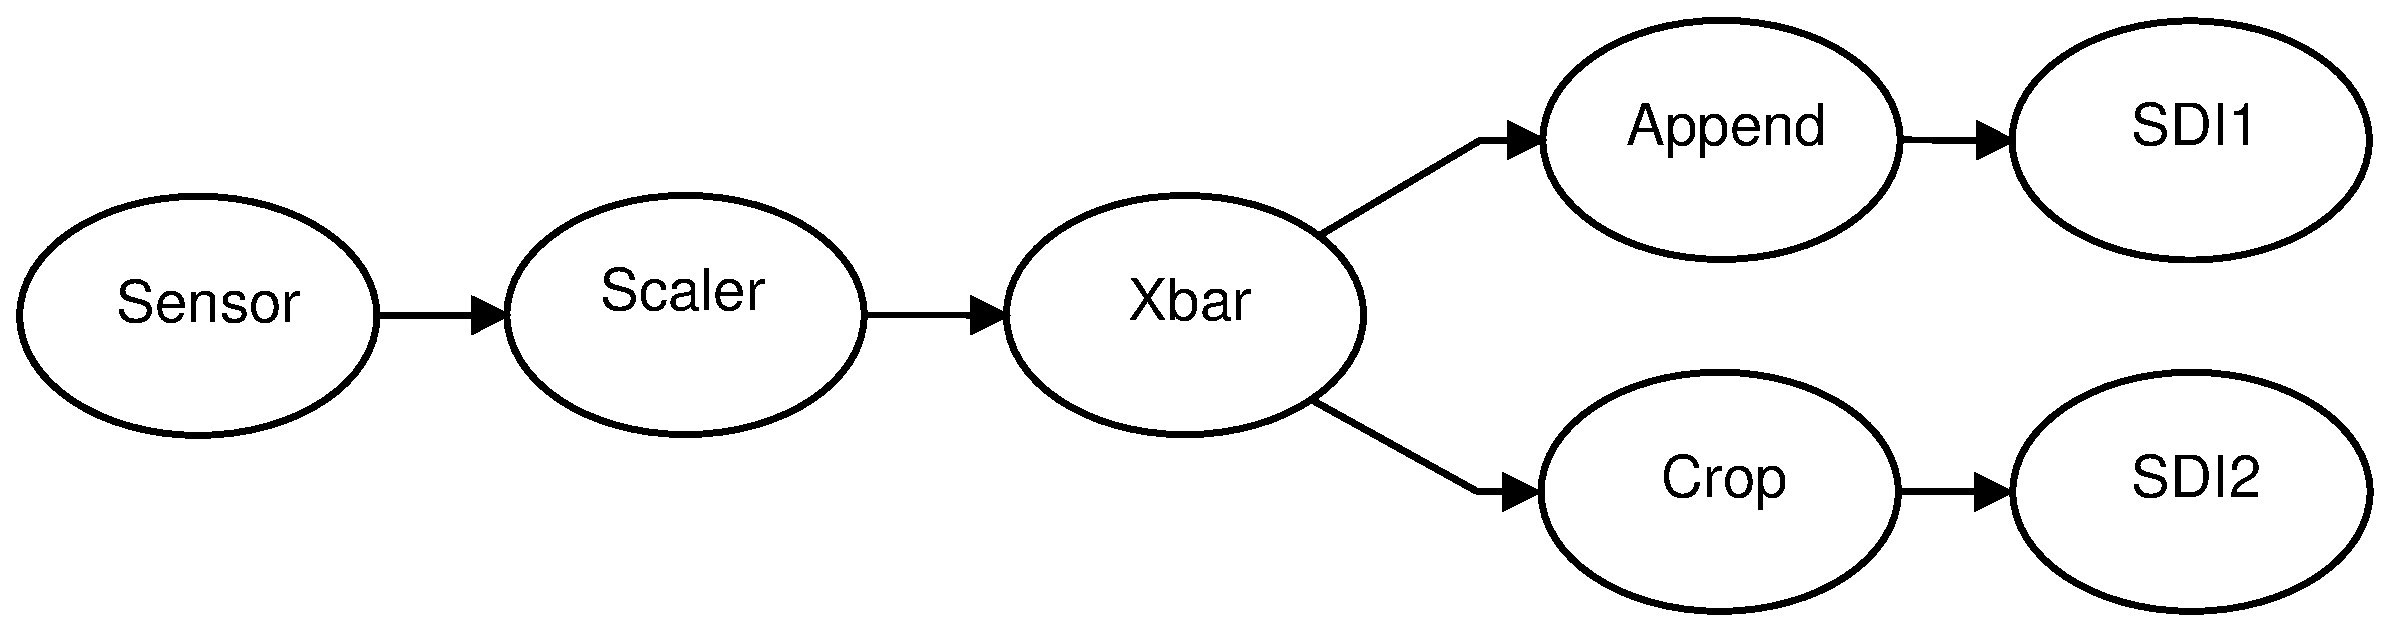
\includegraphics[width = \linewidth]{pictures/Bildkette.eps}
%	\smallskip
%	\caption{Schematische Bildkette}
%	\label{fig:bildkette}
%\end{figure} 

%In der Abbildung \ref{fig:bildkette} sieht man eine schematische Bildkette, die in diesem Bericht zur Veranschaulichung weiter detailliert wird. Das Bild an den \ac{sdi} Ausgängen wird durch verschiedene Module geleitet und angepasst. Auf die Funktionsweise der Module \ac{xbar}, Scaler, Crop sowie Append und die Implementierung wird in den nächsten Unterkapiteln eingegangen.

%\section{Funktionsweise der Module}
%Module: Scaler, Framebuffer, Append, Xbar, Crop, Resize
%Scaler: Berechnung des Bilds aufgrund des angegebenen Skalierungsverhältnis
%Xbar: Verbinden von verschiedenen Pfaden
%Append: Anpassen des Bild auf eine bestimmte Größe, dazufügen
%Crop: Anpassen des Bild auf eine bestimmte Größe, wegschneiden
%Im \ac{FPGA} sind verschiedene Module programmiert und vorkonfiguriert. Um die Kamerasoftware zu vereinfachen werden die Module auch dort angelegt.

%In diesem Abschnitt soll näher auf die Funktionsweise der einzelnen Module eingegangen werden, bevor sich der nächste Abschnitt mit der Programmierung auseinander setzt.

%Im Allgemeinen werden alle Module softwareseitig nur beschrieben, die Algorithmen der einzelnen Module sind im \ac{FPGA} verankert.

%Als erstes wird die \ac{xbar} erläutert. In diesem Modul finden keine Berechnungen statt. Durch entsprechende Konfigurationen kann die \ac{xbar} Bildpfade teilen und auch wieder zusammenfügen.

%Um das Ausgangsbild auf die richtige Größe zu skalieren wird ein Scaler eingesetzt. Hierzu wird dem Scaler ein Skalierungsverhältnis übergeben und das Modul berechnet selbstständig die richtige Ausgangsgröße.

%Die letzten beiden betrachteten Module sind von der grundsätzlichen Idee ähnlich. Durch beide Module soll das Eingangsbild auf eine bestimmte Ausgangsgröße angepasst werden. 
%Der Crop verringert die Eingangsgröße auf die Ausgangsgröße. Im Gegensatz dazu erweitert das Append die Eingangsgröße in dem ein schwarzer Rahmen um das Bild hinzugefügt wird.

%\section{Programmierung der Module}

%Für die Auswahl einer geeigneten Programmiersprache muss berücksichtigt werden, dass jedes Modul über die gleichen Eingangs- und Ausgangsgrößen verfügt. Deswegen bietet sich für \ac{geo} die objektorientierte Programmiersprache C++ an. 

%Um die spezifischen Module möglichst weit zu vereinfachen gibt es vier Grundklassen, die aufeinander aufbauen und im folgenden erklärt werden. Die Eingangsgröße soll später vom Sensor zum SDI durchgereicht werden und die Ausgangsgröße vom SDI zum Sensor. 

%\begin{figure}[!hbtp]
%	\centering
%	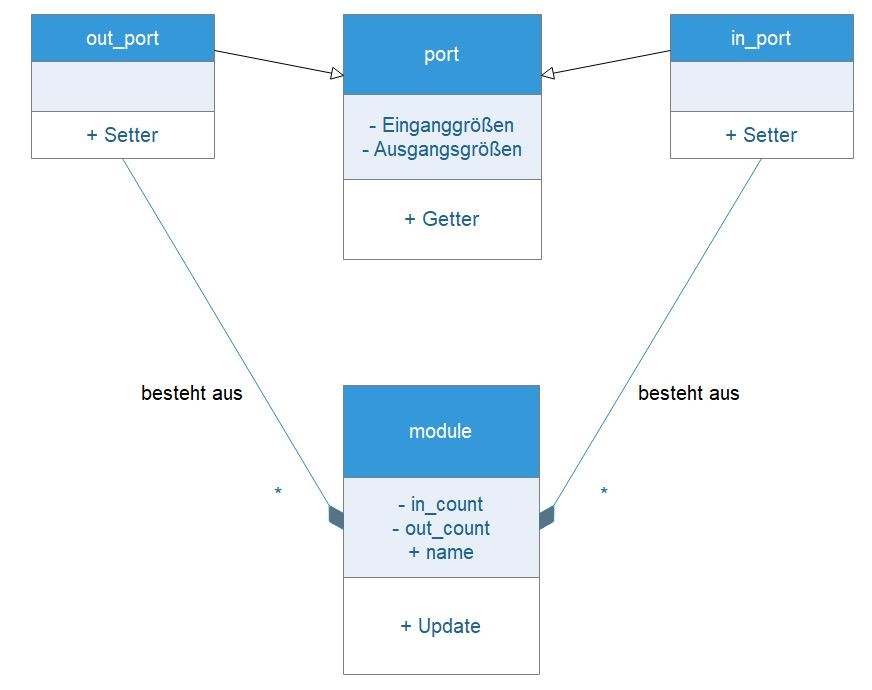
\includegraphics[width = \linewidth]{pictures/uml.jpg}
%	\smallskip
%	\caption{UML Übersicht der Grundklassen}
%	\label{fig:uml}
%\end{figure} 

%Die Klasse Port wird von allen anderen Klassen verwendet (siehe Abbildung \ref{fig:uml}). Hier sind alle Eingangs- und Ausgangsgröße deklariert, sowie alle Getter Funktionen für diese Größen. Im Konstruktor der Klasse muss außerdem ein Portindex mit angegeben werden, welcher auch in den Variablen der Klasse zu finden ist.

%Die beiden friend-Klassen Inport und Outport erben alle Größen und Getter der Port Klasse. Die jeweiligen Setter werden in den Klassen definiert.
%Es wird hier in Eingangs- und Ausgangsport unterschieden, damit nur die richtigen Größen gesetzt werden können. Dadurch, dass die beiden Klassen als friend class definiert sind, können sie auf die Setter der jeweils anderen zugreifen. Für die Updatefunktionen ist dies notwendig damit die Parameter durchgereicht oder berechnete Werte an die Ein- oder Ausgänge geschrieben werden können.

%Die größte Klasse im \ac{geo} ist die Klasse Module. Jedes Modul der Bildkette erbt sein Grundgerüst von dieser Elternklasse. Ein Modul kann aus mehreren Ein- oder Ausgängen bestehen, diese Anzahl wird im Konstruktor angegeben und dementsprechend werden die Ein- und Ausgänge angelegt.

%\begin{minipage}{\textwidth}
%\begin{bash}
%this->in_count = in_count;
%this->out_count = out_count;

%for (i = 0U; i < in_count; i++)
%{
%	in_ports[i] = new in_port(this->name, (geo_port_t)i);
%}

%for (i = 0U; i < out_count; i++)
%{
%	out_ports[i] = new out_port(this->name, (geo_port_t)i);
%}
%\end{bash}
%\captionof{floatcode}{Auszug aus dem Konstruktor der Klasse Module}
%\end{minipage}

%Wie in dem obigen Codeauszug zu sehen werden die privaten Variablen der Klasse auf die angegebene Anzahl von Ein- und Ausgängen gesetzt. Anschließend werden über For-Schleifen die entsprechenden Ports angelegt.

%\begin{figure}[!hbtp]
%	\centering
%	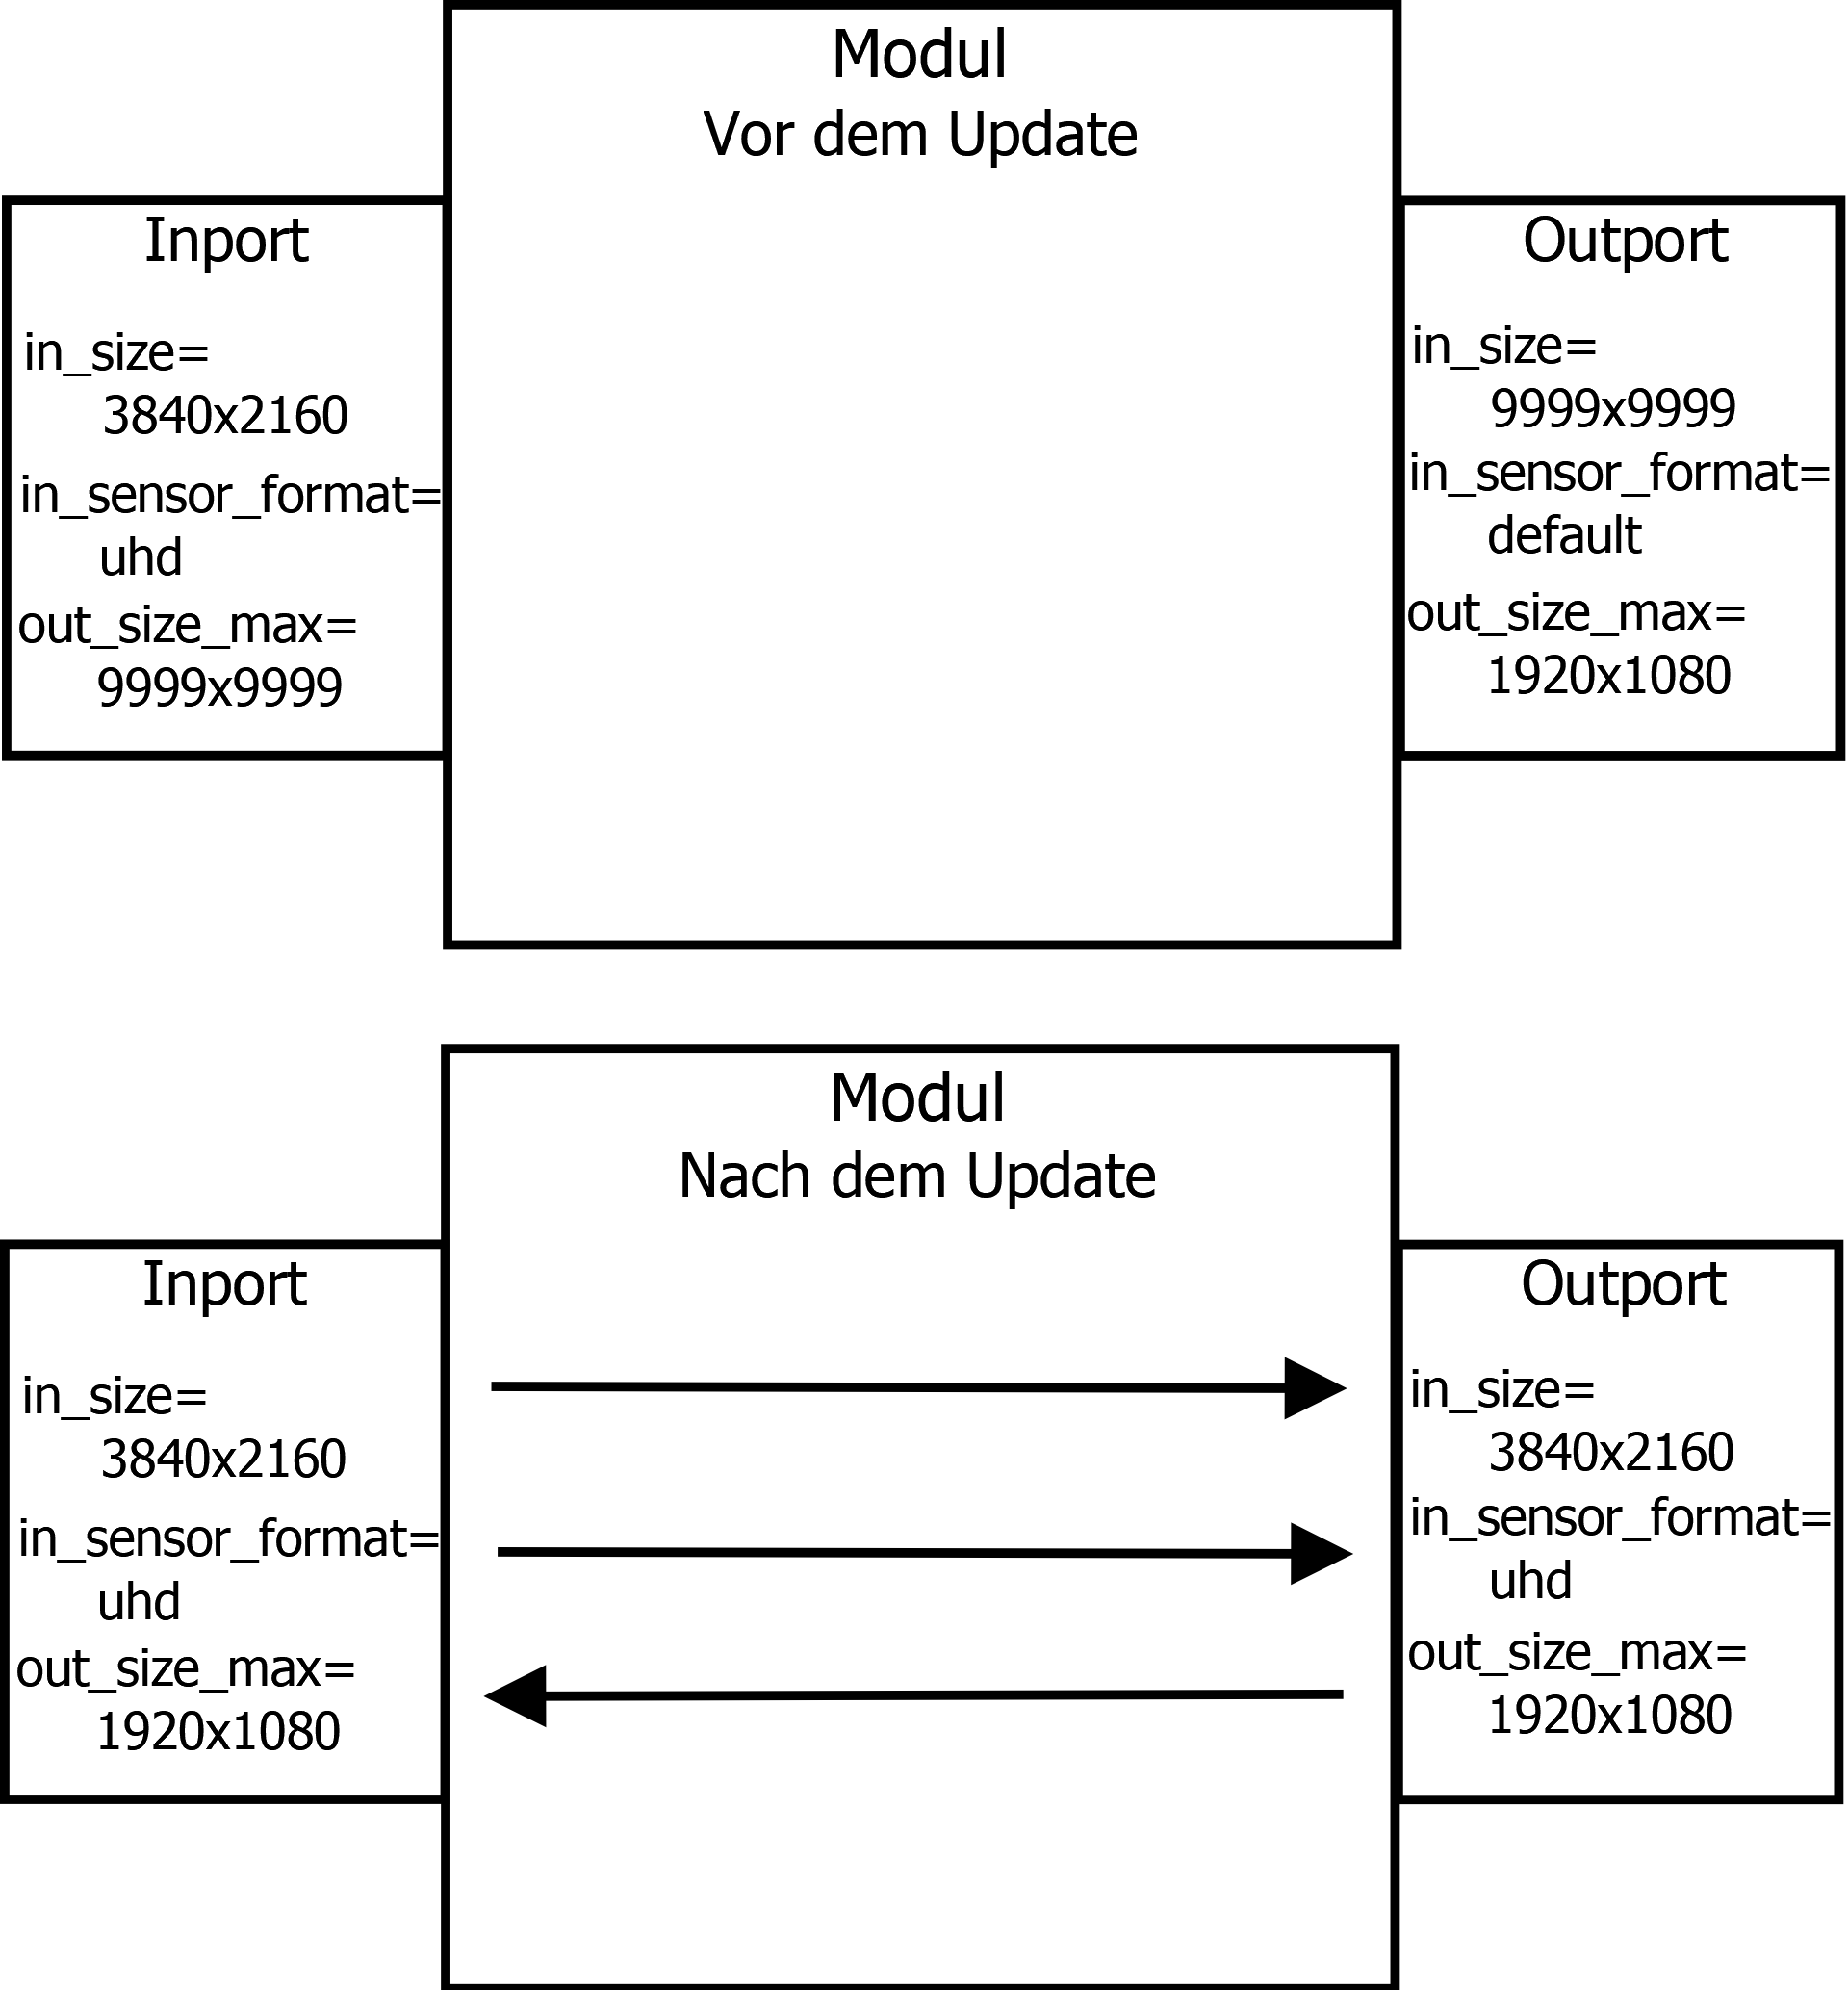
\includegraphics[width = \linewidth]{pictures/update.png}
%	\smallskip
%	\caption{Übersicht der Updatefunktion}
%	\label{fig:update}
%\end{figure} 

%Desweiteren sind in der Klasse auch Updatefunktionen (siehe Abbildung \ref{fig:update}) für jede Größe definiert. Hier werden die Größen am Eingangsport abgefragt und an den Ausgangsport übertragen beziehungsweise am Ausgangsport abgefragt und an den Eingangsport geschrieben. 

%\subsection{\acl{xbar}}
%Das Modul hat eine wichtige Aufgabe in der Kamera. Durch die \acl{xbar} können die Daten aus einem Pfad in mehr Pfade aufgeteilt werden. 

%Damit muss die Updatefunktion der Module Klasse komplett und nicht nur zu Teilen überlagert werden. Hierzu sind ein paar der Ausgangsparameter als Bitmasken angelegt. So wird garantiert, dass auch vor einer \ac{xbar} noch nachvollzogen werden kann, welche Einstellungen an dem Ausgängen vorliegen. Dies ist vor allem bei den nachfolgenden Modulen wichtig, da diese abhängig von den Einstellungen ihre Berechnungen durchführen. 

%\begin{minipage}{\textwidth}
%\begin{bash}
%void set_config(uint32_t config);
%void connect_ports(uint32_t in_port, uint32_t out_port);
%\end{bash}
%\captionof{floatcode}{Deklaration der Konfigurationsfunktionen}
%\end{minipage}

%Die Klasse \ac{xbar} hat zudem zwei Funktionen um die Konfiguration einzustellen. Bei der einen übergibt man eine Bitmaske, welche man aus vorhandenen Defines verodern kann. Die zweite Funktion besteht aus zwei Übergabeparametern, hier gibt man direkt den Eingangs- und Ausgangsport an. Auch die Abfrage der Konfiguration kann über zwei Funktionen stattfinden. Einmal kann man alle Konfigurationen abfragen und der anderen Funktion übergibt man einen Ausgangsport und bekommt den entsprechenden Eingangsport zurück.


%\subsection{Scaler}
%Der Scaler führt Berechnungen aus um das Sensorbild auf die richtige Ausgangsgröße zu skalieren. In der Kamerasoftware wird an dieser Stelle immer nur runterskaliert. 

%Die Klasse hat noch zusätzliche Variablen, diese sind jeweils doppelt vorhanden um die Vertikale und die Horizontale abzubilden. Der Divisor und der Multipikator sind die wichtigsten Parameter. In der Klasse wird die Eingangsgröße durch den Divisor geteilt und anschließend mit dem Multipikator multipliziert. Das Ergebnis wird gerundet und an den Ausgang geschrieben. Diese Berechnungen werden wieder für die Höhe und die Breite des Bildes durchgeführt. Die Variablen werden durch einen Setter gesetzt, allerdings können sie einzeln und unabhängig voneinander abgefragt werden. 

%In dieser Klasse wird nur die Updatefunktion der Elternklasse Module für die Ausgangsgrößen überschrieben. Alle anderen Parameter werden durch das Module durchgereicht und nicht verändert. 

%\subsection{Crop}
%Um den Surround View einstellen zu können wird der Crop notwendig. Wenn diese Einstellung ausgeschalten ist, soll dass Bild am Ausgang anliegen, dass vom Medium aufgezeichnet wird. Hierzu muss das Crop Modul genau den Ausschnitt aus dem Bild ausschneiden, damit liegt am Ausgang das Recordingbild an.

%Auch bei diesem Modul sind nur die Ausgangsgrößen relevant und somit wird hier nur diese Updatefunktion überlagert. Durch die Möglichkeit der Klasse verschiedene Modi einzustellen, werden dort auch entsprechende Berechnungen durchgeführt. Durch die Modi kann man am Ausgang entweder manuell eine Größe einstellen oder die Größe auf die Ausgangsgröße einstellen lassen. Zusätzlich kann man auch das Crop deaktivieren. 

%Eine Besonderheit des Moduls im \ac{FPGA} ist, dass die Ausgangsgrößen teilweise durch eine gerade Zahl teilbar sein muss. Um dies zu garantieren, gibt es in der Klasse Funktionen, die entsprechend die berechneten Größen rundet. 


%\subsection{Append}
%An den Ausgängen sollen unter anderem auch \ac{gui} eingeblendet werden. Dazu wird das Bild kleiner skaliert als der Ausgang und anschließend muss es wieder auf die Ausgangsgröße erweitert werden. Das Append Modul fügt einen schwarzen Rahmen um das Bild, über diesen Rahmen wird die \ac{gui} gelegt. 

%Bei der Klasse kann man verschiedene Modi einstellen. Über die Modi kann man das Bild auf die Ausgangsgröße erweitern, manuell eine Größe einstellen oder das Append Modul außer Betrieb setzen.

%Das Modul überschreibt von der Elternklasse nur die Ausgangsgrößen, da keine anderen neu kalkuliert werden müssen. Des weiteren kann man nicht nur den Modi setzen, sondern natürlich auch eine Ausgangsgröße einstellen. Beim manuellen Modus wird diesen dann eingestellt. 

%Ein anderer Setter ist die Möglichkeit, die Rahmenfarbe einzustellen. Im normalen Betrieb wird nur die Farbe schwarz verwendet, allerdings muss für Entwicklungszwecke die Farbe wählbar sein.

%\section{Einbindung in die Software}
%Um das \ac{geo} in die Kamera einbinden zu können, müssen zwei Aspekte betrachtet werden. Auf der einen Seite muss man die Bildkette auch in der Software abbilden können und auf der anderen Seite muss der Zugriff auf die Module stattfinden.

%\subsection{Softwareseitige Erstellung der Bildkette}
%code anschauen
%Damit die gewünschte Übersichtlichkeit in der Software erreicht wird, muss die Bildkette nicht nur im \ac{FPGA} vorhanden sein, sondern in dem Umfang auch von der Software abgebildet werden.

%Hierzu werden die vorhandenen \ac{FPGA} - Module durch die C++ Klassen abgebildet. Zuallererst werden hier die Module angelegt und im Anschluss werden Ein- und Ausgangsport hintereinander liegender Module verbunden. Damit wird sichergestellt, dass alle Größen von der Quelle bis zur Senke gelangen, bzw. andersherum.


%\subsection{Zugriff auf die Module}
%Da die Kamerasoftware in der Programmiersprache C geschrieben ist, muss eine Ebene geschaffen werden um auf die Funktionen der C++ Module im restlichen Teil der Software zuzugreifen. 

%Die Objekte werden in C++ in einer Liste verwaltet, damit braucht man für den Funktionsaufruf nur den Modulindex und die einzustellende Grüße. 

%\begin{minipage}{\textwidth}
%\begin{bash}
%void geoif_append_set_size_append(uint32_t module_idx, struct size size_append)
%{
%	append *var;
%	if (geo_system == NULL)
%	{
%		error_msg(EH_WARNING, 
%			"Geo system not initialised.");
%		return;
%	}
%	if (geo_system->get_module(module_idx) == NULL)
%	{
%		error_msg(EH_WARNING, 
%			"No module exists index \%u", module_idx);
%		return;
%	}
%	var = (append *)(geo_system->get_module(module_idx));
%	if (var == NULL)
%	{
%		error_msg(EH_WARNING, 
%			"Module at index \%u is not append.",
%			module_idx);
%		return;
%	}

%	a->set_size_append(size_append);
%}
%\end{bash}
%\captionof{floatcode}{Funktion eines Appends für C }
%\end{minipage}

%Wie man in dem obigen Codebeispiel sieht, kann die Kamerasoftware nicht direkt auf die Module zugreifen sondern geht über eine Extrafunktion. Bei dieser und allen weiteren Funktionen wird als Erstes überprüft, ob das Modul an diesem Index, dem der Funktion entspricht. Wenn dieses nicht der Fall ist, wird die Funktion verlassen. Bei einer Übereinstimmung der Module wird in der nächsten Zeile die entsprechende Größe in diesem Modul gesetzt.

%Am Ende werden die Module in der zuvor definierten Reihenfolge geupdatet und damit sind in jedem Modul die richtigen Größen und Werte.

%\subsection{Übertragen der Größen in den \ac{FPGA}}
%Am Ende müssen die in dem \ac{geo} eingestellten Größen in die Module des \ac{FPGA}s übertragen werden. Hierzu werden die richtigen Module auf Software- und Hardwareseite zusammen aufgerufen. Die Größen des Moduls werden aus dem \ac{geo} entnommen und über entsprechende Hardwarefunktionen in die Register des \ac{FPGA}s geschrieben. An diesem Punkt findet allerdings keine Überprüfung auf die Richtigkeit des Moduls statt, sondern lediglich die Kontrolle, ob dieses im \ac{geo} und im \ac{FPGA} existiert.


